\section{When does aggregation pay: measurements}\label{sec:pay-meas}

\subsection{Step ablation on real data}\label{sec:meas-kreal}
Table~\ref{tab:kreal} separates the three effects the batteries of
Section~\ref{sec:exp} mix: the guard and away fallback (guarded $k{=}1$
against plain MDM), aggregation ($k{=}16$ and the adaptive size of
Section~\ref{sec:adaptive} against guarded $k{=}1$), and the
comparison with BPCG, all in isolated runs with a time split. Two
effects separate. The guard and away fallback alone cut plain pairwise
FW's iterations $1.4$--$2.7\times$ and its time by at most $1.3\times$
(a tie on gisette and ijcnn1); aggregation cuts iterations a further
$3.8$--$7.0\times$, which buys wall-clock only where per-iteration
$O(n)$ work, not column computation, dominates: $1.8$--$2.4\times$
over guarded $k{=}1$ on the four kernel cells ($3.8$--$6.1\times$ over
BPCG) and nothing on gisette.

\begin{table}[htbp]\centering\scriptsize\setlength{\tabcolsep}{3.5pt}
\caption{Step ablation on real data with a time split, isolated runs
(\texttt{src/step\_profile.py}: three seeds, each configuration alone
in its own process on an otherwise idle machine, with the final code):
the gisette $L_2$
margin ($C{=}1$, $d{=}5{,}000$) and the four kernel $L_2$ cells of
Table~\ref{tab:regime}. MDM is plain
pairwise FW (single transfers, no guard, no fallback, the same
prioritised receiver search and schedule as the other rows); guarded $k{=}1$
is Algorithm~\ref{alg:block} with a single pair (guard and case-(b)
fallback active); auto is the adaptive block size of
Section~\ref{sec:adaptive} (median $k$ over the run given); BPCG as in
Table~\ref{tab:bpcg}. Split of the ETA time: scan = the score scan and
pair selection; col = Gram or kernel column computation; step = the
step itself (block assembly, guard, line search, cache and score
update); rest = certificate and bounds. Drops = away fallbacks that
removed a support index. Every run converged to the certified gap with
identical distance and accuracy per dataset and seed. Peak resident
memory: $0.74$\,GB on gisette, $0.48$--$0.93$\,GB for ETA and
$0.66$--$1.29$\,GB for BPCG on the kernel cells. The gisette column
time varied by $\pm15\%$ between three isolated runs of the same
trajectory on the same machine ($26$--$35$\,s;
\texttt{results/step\_profile\{,2,3\}.json}), more than the $8\%$
that separates its fastest and slowest rows here, so its rows should be
read as a tie.}\label{tab:kreal}
\begin{tabular}{llrrrrrrrrr}\toprule
instance & step & $k$ & time (s) & scan & col & step & rest & iterations & columns & drops \\\midrule
gisette $L_2$ & MDM & 1 & $29.4\pm0.2$ & 0.2 & 26.0 & 1.0 & 2.1 & 4,946 & 1,300 & 0 \\
gisette $L_2$ & guarded & 1 & $30.1\pm0.3$ & 0.2 & 26.6 & 1.8 & 1.5 & 3,471 & 1,334 & 82 \\
gisette $L_2$ & block & 16 & $31.9\pm0.5$ & 0.1 & 29.7 & 1.7 & 0.4 & 831 & 1,480 & 301 \\
gisette $L_2$ & auto & 9 & $30.9\pm1.4$ & 0.1 & 28.8 & 1.6 & 0.5 & 986 & 1,451 & 194 \\
gisette $L_2$ & BPCG & --- & $29.8\pm0.5$ & & & & & 10,470 & 1,322 & 87 \\
\midrule
ijcnn1 kernel $L_2$ & MDM & 1 & $10.3\pm0.5$ & 1.3 & 0.9 & 2.9 & 5.2 & 12,796 & 4,520 & 0 \\
ijcnn1 kernel $L_2$ & guarded & 1 & $9.7\pm0.4$ & 0.8 & 0.8 & 4.5 & 3.6 & 6,118 & 4,514 & 14 \\
ijcnn1 kernel $L_2$ & block & 16 & $5.3\pm0.8$ & 0.2 & 0.8 & 3.3 & 1.0 & 1,396 & 4,590 & 98 \\
ijcnn1 kernel $L_2$ & auto & 8 & $4.7\pm0.6$ & 0.3 & 0.7 & 2.6 & 1.1 & 1,734 & 4,570 & 75 \\
ijcnn1 kernel $L_2$ & BPCG & --- & $19.9\pm2.2$ & & & & & 18,034 & 4,512 & 19 \\
\midrule
w8a kernel $L_2$ & MDM & 1 & $8.8\pm0.8$ & 0.9 & 2.8 & 2.2 & 2.9 & 11,461 & 3,587 & 0 \\
w8a kernel $L_2$ & guarded & 1 & $7.3\pm1.2$ & 0.4 & 2.7 & 2.7 & 1.4 & 4,243 & 3,581 & 8 \\
w8a kernel $L_2$ & block & 16 & $4.0\pm0.2$ & 0.1 & 2.4 & 1.2 & 0.3 & 603 & 3,591 & 50 \\
w8a kernel $L_2$ & auto & 10 & $3.8\pm0.2$ & 0.1 & 2.3 & 1.1 & 0.3 & 756 & 3,590 & 40 \\
w8a kernel $L_2$ & BPCG & --- & $17.5\pm2.0$ & & & & & 12,342 & 3,577 & 12 \\
\midrule
a9a kernel $L_2$ & MDM & 1 & $31.5\pm1.6$ & 3.4 & 4.5 & 7.3 & 16.4 & 22,901 & 7,607 & 0 \\
a9a kernel $L_2$ & guarded & 1 & $24.2\pm2.1$ & 1.9 & 3.9 & 9.7 & 8.8 & 9,879 & 7,611 & 27 \\
a9a kernel $L_2$ & block & 16 & $10.0\pm0.5$ & 0.3 & 3.8 & 4.2 & 1.7 & 1,489 & 7,616 & 35 \\
a9a kernel $L_2$ & auto & 13 & $10.0\pm0.5$ & 0.4 & 3.7 & 4.0 & 1.9 & 1,641 & 7,607 & 26 \\
a9a kernel $L_2$ & BPCG & --- & $60.7\pm1.2$ & & & & & 28,653 & 7,605 & 24 \\
\midrule
covtype kernel $L_2$ & MDM & 1 & $39.5\pm1.4$ & 4.4 & 2.9 & 9.6 & 22.6 & 26,756 & 9,069 & 0 \\
covtype kernel $L_2$ & guarded & 1 & $33.4\pm2.2$ & 2.6 & 2.5 & 13.7 & 14.6 & 12,544 & 9,069 & 12 \\
covtype kernel $L_2$ & block & 16 & $17.4\pm0.5$ & 0.9 & 2.5 & 9.4 & 4.6 & 3,336 & 9,074 & 26 \\
covtype kernel $L_2$ & auto & 7 & $16.8\pm1.7$ & 1.0 & 2.4 & 7.9 & 5.5 & 4,154 & 9,071 & 19 \\
covtype kernel $L_2$ & BPCG & --- & $85.3\pm4.5$ & & & & & 38,422 & 9,065 & 15 \\
\bottomrule\end{tabular}\end{table}

The guarded single pair already halves the iterations of plain MDM on
ijcnn1 ($1.4\times$ on gisette): the drop steps it takes (on $0.1$--$2.4\%$
of its iterations) are what plain pairwise FW replaces by capped
swaps. Blocks then cut iterations a further $3.8$--$7.0\times$
(isolated seed-0 runs at $k{=}4$ are in Table~\ref{tab:diag}: within
$31\%$ of $k{=}16$ in time on every cell). Away fallbacks that drop an index occur on
$0.1$--$36\%$ of guarded iterations, and their share grows with $k$:
larger blocks add more indices per iteration, and the drops remove
them. The time split says where fewer iterations buy time. On gisette,
$88$--$93\%$ of every configuration's time is Gram-column computation
($O(nd)$ per new receiver, $d{=}5{,}000$), so MDM, guarded $k{=}1$,
block $k{=}16$, the adaptive size and BPCG all lie within $8\%$ of one
another at $29$--$32$\,s, inside the between-run variation of the
column time. On ijcnn1 the columns cost
about $1$\,s and the rest is per-iteration $O(n)$ work: the score
update and line search inside the step, the certificate in the
remainder, and least of all the scan itself. That work falls with the
iteration count, though not in proportion, because a block step updates
the scores with up to $k'$ columns; the net effect on ijcnn1 is
$1.9\times$ over MDM and $3.8\times$ over BPCG at $k{=}16$, and
$2.2\times$ and $4.2\times$ with the adaptive size, which settles at
$k{=}7$--$8$, the $k^*$ of Section~\ref{sec:pay-meas}; the other three
kernel cells behave alike (Table~\ref{tab:kreal}).

\begin{table}[htbp]\centering\scriptsize
\caption{BPCG \citep{tsuji2022} versus block ETA ($k{=}16$) on the same
objective with the same certificate ($\varepsilon{=}10^{-3}$), the same
column cache and the same 600\,s cap (\texttt{src/bpcg\_baseline.py},
solver \texttt{src/bpcg.py}); three seeds,
run concurrently with Table~\ref{tab:regime}; Table~\ref{tab:kreal}
gives the isolated reruns. Every cell converged; distances agree per
cell to five digits and test accuracies to $10^{-4}$. Columns are
kernel or Gram columns computed; drops count BPCG's capped
local steps and ETA's away drops.}\label{tab:bpcg}
\begin{tabular}{llrrrr}\toprule
cell & solver & time (s) & iterations & columns & drops \\\midrule
gisette $L_2$, $C{=}1$ & BPCG & $34.2\pm20.4$ & 10,470 & 1,322 & 87 \\
gisette $L_2$, $C{=}1$ & ETA & $34.3\pm15.0$ & 831 & 1,480 & 301 \\
\midrule
gisette KL2 & BPCG & $213\pm28$ & 8,702 & 3,641 & 3 \\
gisette KL2 & ETA & $83.9\pm19.0$ & 251 & 3,653 & 4 \\
w8a KL2 & BPCG & $22.3\pm5.8$ & 12,342 & 3,577 & 12 \\
w8a KL2 & ETA & $5.0\pm2.2$ & 603 & 3,591 & 50 \\
a9a KL2 & BPCG & $65.4\pm5.7$ & 28,653 & 7,605 & 24 \\
a9a KL2 & ETA & $11.7\pm2.2$ & 1,489 & 7,616 & 35 \\
covtype KL2 & BPCG & $90.6\pm11.2$ & 38,422 & 9,065 & 15 \\
covtype KL2 & ETA & $20.3\pm1.1$ & 3,336 & 9,074 & 26 \\
ijcnn1 KL2 & BPCG & $20.2\pm1.6$ & 18,034 & 4,512 & 19 \\
ijcnn1 KL2 & ETA & $5.9\pm1.1$ & 1,396 & 4,590 & 98 \\
\bottomrule\end{tabular}\end{table}

BPCG here is the blended pairwise step of \citet{tsuji2022} on the
$nm$ product atoms $v_i-w_j$ of $Z$, with product-atom capacities, the
separable LMO of Lemma~\ref{lem:sep}, exact line searches and the
certificate of Lemma~\ref{lem:gapid}; its scores are maintained from
the same cached columns, so column counts are comparable, but its
active set is a Python-level dictionary over product atoms, and on that
parametrisation it needs $1.1$--$2.1\times$ more iterations than even
plain MDM with side transfers (gisette $10{,}470$ vs $4{,}946$; ijcnn1
$18{,}034$ vs $12{,}796$). The $11$--$35\times$ iteration ratio and the
$2.5$--$5.6\times$ wall-clock ratio against block ETA therefore compare
parametrisation and implementation as well as step rules; a BPCG on the
side-transfer parametrisation is listed in Section~\ref{sec:limits}.
The block's fewer scans buy time where scans dominate (KL2) and nothing
where columns do (gisette $L_2$).

\subsection{Per-step measurements}\label{sec:meas}

Every quantity in Proposition~\ref{prop:ratio}, the cost model and
Theorem~\ref{thm:ident} was recorded on the five real cells of
Table~\ref{tab:regime} (gisette $L_2$ and the kernel $L_2$ cells of
ijcnn1, w8a, a9a and covtype, seed 0; \texttt{src/block\_diagnostics.py}, one process at a time on an
otherwise idle machine, $k\in\{1,4,16,32\}$). At every block step the
solver logs $\Delta_B$, $\Delta_1$, $Q$, $\chi$, the candidate taken,
the capped pairs, the column misses, the support size and a time split
of the step next to a dry-run timing of the single MDM update from the
same state. Table~\ref{tab:diag} fits the model per cell:
$\hat\eta=(\chi-1)/(k'-1)$ (median over the block calls with pair 1
uncapped; a \emph{block call} is one side's execution of
Algorithm~\ref{alg:block}, up to two per iteration), $a$ and $b$ by
least squares of the non-column time per iteration on $k$,
$c_{\mathrm{col}}$ as column time per column.

\begin{table}[t]\centering\scriptsize\setlength{\tabcolsep}{4pt}
\caption{The timing model fitted per cell (seed 0; the twenty
configurations run one after the other in a single process with the
per-step instrumentation on, which adds $5$--$34\%$ to the times of
Table~\ref{tab:kreal}; the coefficients describe these instrumented
runs). $\hat\eta$ is the median over $k\in\{4,16,32\}$; the $k=16$ and
$k=32$ estimates agree within $0.01$ and the $k=4$ estimate within
$0.04$ of them (gisette $0.04/0.08/0.07$, w8a $0.20/0.17/0.16$). $k^*$
from \eqref{eq:kstar} with $\hat\eta$ in place of $\eta$. Times for $k=1/4/16/32$; ``column share'' is the
fraction of the $k{=}16$ run spent computing columns; the last column is
the speed-up of the best $k$ over the guarded single pair.}\label{tab:diag}
\begin{tabular}{lrrrrrlrr}\toprule
cell & $\hat\eta$ & $a$ (ms) & $b$ (ms) & $c_{\mathrm{col}}$ (ms) & $k^*$ & time (s), $k=1/4/16/32$ & column share & best $k$ vs $k{=}1$ \\\midrule
% rows generated by src/block_diag_fig.py --inp results/block_diag3.json
gisette $L_2$ & 0.07 & 1.3 & 0.080 & 21.30 & 14 & 33.0 / 29.2 / 33.9 / 38.0 & 93\% & 1.1$\times$ (4) \\
ijcnn1 KL2 & 0.26 & 1.7 & 0.098 & 0.23 & 7 & 11.6 / 6.1 / 6.1 / 7.6 & 17\% & 1.9$\times$ (4) \\
w8a KL2 & 0.17 & 1.3 & 0.077 & 0.88 & 9 & 9.7 / 5.3 / 4.4 / 4.6 & 64\% & 2.2$\times$ (16) \\
a9a KL2 & 0.11 & 2.5 & 0.111 & 0.62 & 13 & 30.5 / 14.2 / 10.8 / 11.7 & 41\% & 2.8$\times$ (16) \\
covtype KL2 & 0.29 & 2.8 & 0.102 & 0.35 & 8 & 38.9 / 21.0 / 18.2 / 21.7 & 17\% & 2.1$\times$ (16) \\
\bottomrule\end{tabular}\end{table}

\begin{figure}[t]\centering
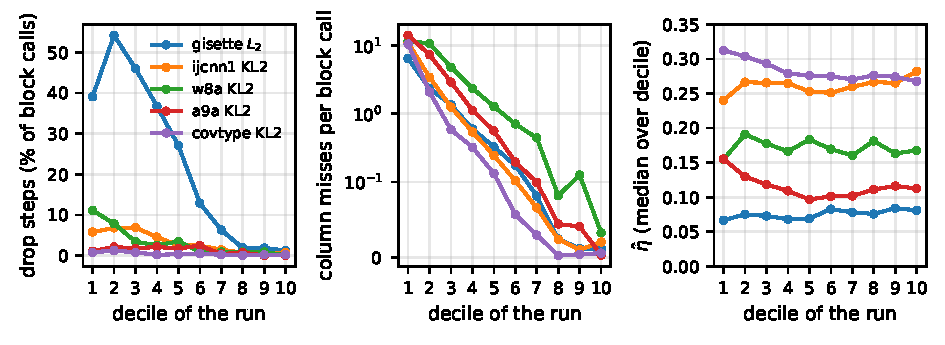
\includegraphics[width=\linewidth]{figs/fig_diag.pdf}
\caption{Along the run at $k=16$ (deciles of the iteration count, one
line per cell): fraction of block calls that are drops, column misses per
block call, and the effective correlation $\hat\eta$. Drops and misses
are paid while the support is built and become rare once it has
settled, the shape Theorem~\ref{thm:ident} describes; $\hat\eta$ is
constant along the run.}\label{fig:diag}
\end{figure}

Four facts follow.
\begin{itemize}\setlength\itemsep{0pt}
\item \emph{$\hat\eta$ is stable on each cell.} The effective
correlation does not move with $k$ nor along the run
(Figure~\ref{fig:diag}, right), although it is a statistic of the
iterates and the pairing rule rather than of the data alone; it is $0.07$ on
gisette, $0.11$ on a9a, $0.17$ on w8a, $0.26$ on ijcnn1 and $0.29$ on
covtype, and $0.001$ on the synthetic instance of
Table~\ref{tab:adaptive} at $d{=}1{,}000$. The mean relative pair gain
$Q/k'=(1/k')\sum_j\Delta_j/\Delta_1$ (median $Q$ over the run's block
calls with pair 1 uncapped, divided by the mean number of retained
pairs) is $0.92$--$0.98$ at $k=4$, $0.83$--$0.98$ at $k=16$ and
$0.78$--$0.88$ at $k=32$ (Table~\ref{tab:assump} lists the $k=16$
values): the useful progress beyond the leading pair is never the
limit, the loss to combination is. The measured gain ratios (median
$\max(\Delta_B,\Delta_1)/\Delta_1$ over the same calls: $3.4/6.9/7.5$ on
gisette and $2.1/2.8/3.0$ on ijcnn1 at $k=4/16/32$) follow
$k/(1+\hat\eta(k-1))$ within $35\%$; on ijcnn1 they saturate near
$1/\hat\eta=3.8$, on gisette they are still rising at $k=32$ ($7.5$
against $1/\hat\eta=14$).
\item \emph{$k^*$ is $7$--$14$ on every cell}, because $a/b$ is
$16$--$28$ throughout and $\hat\eta\in[0.07,0.29]$: a fixed block size
of $8$--$16$ is within $16\%$ of the best measured time on all five
cells ($k{=}16$ against the best size: $16\%$ on gisette, under $1\%$
elsewhere; $k{=}4$ is within $31\%$ of $k{=}16$ on every cell), so the
untuned $k=16$ of Section~\ref{sec:exp} never lost to another size by
more than that.
\item \emph{The wall-clock gain is bounded by the single pair's column
share.} The block cannot touch the column term of the timing model
($N_{\mathrm{cols}}$ varies by under $20\%$ across $k$ on every cell),
so no block size can beat the guarded single pair by more than the
reciprocal of the fraction of that run spent on columns ($T_1/T_{\mathrm{col}}$:
$1.1$ on gisette, $2.4$ on w8a, $5.5$ on a9a, $11$--$12$ on ijcnn1 and
covtype). The measured speed-ups are $1.1\times$ on gisette,
$2.2\times$ on w8a, $2.8\times$ on a9a and $1.9$--$2.1\times$ on ijcnn1
and covtype, where the iteration gain has saturated at $1/\hat\eta$
long before the column bound matters. (The share of the $k{=}16$ run
in the table is not a bound: w8a's $2.2\times$ exceeds $1/0.64$.) The
model's time predictions, $aT+b\sum_tk'_t+c_{\mathrm{col}}N_{\mathrm{cols}}$
with the fitted coefficients, are within $14\%$ of the measurements at
$k\le4$ and within $5\%$ on gisette at every $k$; at $k=16$--$32$ on
the kernel cells they are $24$--$50\%$ too high, because the runs need
fewer iterations than the one-state ratio predicts: the trajectory
effect is in the block's favour, and the model is conservative.
\item \emph{Drops are front-loaded} (Figure~\ref{fig:diag}, left). On
gisette at $k=16$ half of the block calls in the first three deciles are
drops and $1$--$2\%$ in the last three; the kernel cells show the same
shape at lower levels; nearly every case-(b) call is a drop, so the
best-of-four branch is rare. Column misses follow the same curve, so on
column-bound cells the whole column bill is paid during identification
whichever $k$ is used. Total drops per point of one class's final
support are $0.13/0.13/0.48/0.69$ on gisette and $0.003$--$0.10$ on the
kernel cells for $k=1/4/16/32$: growing with $k$, and an order of
magnitude more frequent on the sparse linear cell, where fresh
receivers of small weight become the worst donor at once. On a9a and
covtype the drop fraction is flat over the first six deciles rather
than front-loaded; the shape of Theorem~\ref{thm:ident} is clearest on
gisette, ijcnn1 and w8a.
\end{itemize}
\begin{table}[t]\centering\scriptsize
\caption{The theorem's assumptions against the measured mechanism at
$k=16$ (seed 0; \texttt{src/block\_diagnostics.py} on a second machine,
with iteration and drop counts identical to the runs of
Table~\ref{tab:diag}; its $\hat\eta$ differs from Table~\ref{tab:diag}
in the second decimal because it is the $k=16$ median alone rather than
the median over $k\in\{4,16,32\}$). Over the
block calls with every retained pair uncapped: median maximum absolute
pairwise cosine of the retained directions (the $\eta$ of
Proposition~\ref{prop:ratio}), median minimum relative pair gain (its
$\beta_{\mathrm{flat}}$), and the lower bound the proposition then
guarantees for the guarded ratio $\max(\Delta_B,\Delta_1)/\Delta_1$,
$(1+\beta_{\mathrm{flat}}(k'-1))/(1+\eta(k'-1))$ (column ``bound''); against
the effective correlation $\hat\eta$, the mean relative pair gain
$Q/k'$, the model ratio $k'/(1+\hat\eta(k'-1))$ and the measured median
of $\max(\Delta_B,\Delta_1)/\Delta_1$, the last three over the block
calls with pair 1 uncapped.}\label{tab:assump}
\begin{tabular}{lrrrrrrrr}\toprule
cell & all pairs uncapped & $\max|\cos|$ & $\beta_{\mathrm{flat}}$ & bound & $\hat\eta$ & $Q/k'$ & model & measured \\\midrule
gisette $L_2$ & 43\% & 0.33 & 0.53 & 1.5 & 0.08 & 0.98 & 7.4 & 6.9 \\
ijcnn1 KL2 & 73\% & 0.42 & 0.80 & 1.8 & 0.26 & 0.89 & 3.2 & 2.8 \\
w8a KL2 & 76\% & 0.33 & 0.77 & 2.1 & 0.17 & 0.88 & 4.4 & 3.6 \\
a9a KL2 & 89\% & 0.28 & 0.70 & 2.2 & 0.12 & 0.83 & 5.8 & 4.6 \\
covtype KL2 & 96\% & 0.42 & 0.82 & 1.8 & 0.28 & 0.91 & 3.0 & 2.7 \\
\bottomrule\end{tabular}\end{table}

\emph{The theorem's constants are not what the mechanism runs on.}
Table~\ref{tab:assump} records the assumptions of
Proposition~\ref{prop:ratio} on the real cells. The maximum pairwise
cosine is $0.28$--$0.42$ on every cell, so the $\eta$ of the proposition
does not distinguish the cells at all, whereas the effective correlation
$\hat\eta$ spans $0.07$--$0.29$ and does; the minimum relative gain is
$0.53$--$0.82$; and at $k=16$ only $43$--$96\%$ of the block calls have all
pairs uncapped, so the proposition applies to a minority of the calls on
gisette. The lower bound the proposition guarantees for the guarded
ratio from these constants is $1.5$--$2.2$, against measured medians of
$2.7$--$6.9$ (the bound is an inequality, so the gap is slack, not a
contradiction). The exact identity $Q/\chi$ evaluated on the same calls
gives $7.3/2.9/3.9/4.8/2.8$ against the measured $6.9/2.8/3.6/4.6/2.7$;
the ``model'' column, $k'/(1+\hat\eta(k'-1))$, which replaces $Q$ by
$k'$, is $7$--$26\%$ high. Both reproduce the measurement to within the
spread because they use the $\gamma$-weighted aggregate in which the
cross terms largely cancel, not the worst pair. The right reading of
Proposition~\ref{prop:ratio} is therefore its first, exact, half; the
$\eta$-diverse, $\beta_{\mathrm{flat}}$-flat bound is a worst case that real blocks beat
by a factor of $1.5$--$4.6$.

The measurements are from one seed per cell and the fits are
retrospective (the coefficients are estimated from the same four runs
they describe); the ratios they support (Tables~\ref{tab:kreal}
and~\ref{tab:bpcg}) are reproduced across three seeds in isolated runs,
and Section~\ref{sec:adaptive} is the prospective test. On the
identification mechanism the figure is consistent with
Theorem~\ref{thm:ident} but does not verify it: the theorem's thresholds
$H_{\mathrm{id}},H_{\mathrm w}$ lie below the stopping tolerance of
these runs, and late drops, though rare, do occur. Section~\ref{sec:ident-check}
tests the theorem where its constants can be computed.

\subsection{An adaptive block size}\label{sec:adaptive}

Every quantity in \eqref{eq:kstar} is observable while the solver runs:
$\chi$ is computed by the guard at every block step, so
$\hat\eta=(\chi-1)/(k'-1)$ costs nothing, and $a/b$ is a property of
the implementation ($16$--$28$ in Table~\ref{tab:diag}). The released
code therefore offers \texttt{block\_size='auto'}: every $50$ iterations
it sets $k$ to $\sqrt{(a/b)(1-\hat\eta)/\hat\eta}$, clipped to $[1,k_{\max}]$,
with $\hat\eta$ the median over the window's block steps with $k'>1$
(when fewer than five such steps exist, as at $k=1$, the rule doubles
$k$ to obtain a signal; a non-positive $\hat\eta$ is floored at $10^{-3}$
before the square root, which sends $k$ to $k_{\max}$), and halves $k$ instead when
more than $10\%$ of the window's block calls had their leading pair
capped (drops are outrunning the support). Guard and fallback are
untouched, so Theorem~\ref{thm:linear} applies with $k_{\max}$ in the
drop bound. The rule's form, its window, $k_{\max}=32$ and the ratio
$a/b=20$ were set from the analysis of the two pilot cells (gisette,
ijcnn1); on a run the rule reads only its own window's $\chi$ values,
never the per-cell $\hat\eta$ of Table~\ref{tab:diag}, which is a
retrospective median over three complete runs and enters nothing but
the fitted $k^*$ column of that table. We do not call the other three
cells a prospective test: the $k$-sweeps on w8a, a9a and covtype were
on disk before the rule was committed, and the repository cannot
establish that the constants were fixed without sight of them. They
are cells not used to set the constants, and the check is whether the
rule's wall-clock on them matches the fixed sizes run under the same
protocol (Table~\ref{tab:kreal}). It does: the rule settles at $k=10$,
$13$ and $7$ (the retrospectively fitted $k^*$ are $9$, $13$, $8$) and
takes $3.8\pm0.2$, $10.0\pm0.5$ and $16.8\pm1.7$\,s against
$4.0\pm0.2$, $10.0\pm0.5$ and $17.4\pm0.5$\,s for $k{=}16$, a tie
within CI on every cell, as it is on the two pilot cells ($k{=}9$ then
$15$ on gisette; $k{=}7$--$8$ on ijcnn1, $4.7\pm0.6$ against
$5.3\pm0.8$\,s). The rule's value is that it removes the parameter,
not that it beats a well-chosen fixed size. Table~\ref{tab:adaptive} tests it where
$\eta$ actually varies: synthetic $L_2$ instances ($n{=}2{,}000$ per
class, $C{=}1$) whose transfer directions decorrelate as the dimension
grows, so that $\hat\eta$ falls from $0.31$ at $d{=}20$ to below
$0.002$ at $d\ge300$. The rule tracks $k^*$ across two orders of
magnitude of $\hat\eta$ and is within $0.14$\,s ($14\%$) of the best
fixed size at $d{=}20$ and within $0.1$\,s elsewhere, the resolution of
these short single-seed runs.

\begin{table}[t]\centering\scriptsize
\caption{Adaptive block size on synthetic $L_2$ instances of varying
directional diversity (one process, seed 0, $a/b$ set to $20$,
$k_{\max}=32$). Times for guarded $k{=}1$ and fixed $k=4/16/32$; ``auto''
reports the size the rule settled on and its time.}\label{tab:adaptive}
\begin{tabular}{rrrrrrrr}\toprule
$d$ & $\hat\eta$ & $k^*$ & $k{=}1$ (s) & $k{=}4$ & $k{=}16$ & $k{=}32$ & auto: $k$, time (s) \\\midrule
20 & 0.31 & 7 & 1.3 & 1.0 & 1.1 & 1.3 & 6, 1.1 \\
50 & 0.10 & 13 & 2.1 & 1.2 & 1.0 & 1.3 & 12, 1.1 \\
100 & 0.03 & 24 & 3.5 & 1.8 & 1.1 & 1.2 & 24, 1.1 \\
300 & 0.00 & $>32$ & 1.7 & 0.7 & 0.4 & 0.4 & 32, 0.4 \\
1,000 & 0.00 & $>32$ & 1.5 & 0.9 & 0.7 & 0.7 & 32, 0.7 \\
\bottomrule\end{tabular}\end{table}

\subsection{Numerical check of Theorem~\ref{thm:ident}}\label{sec:ident-check}

The theorem's constants are computable on small instances. For $40$
random hard-margin instances ($d=4$, ten points per class, Gaussian
clouds $2.5$ apart) the SLSQP reference gives $z^*$, the faces, $\tau$,
$\alpha_{\min}$, $d_{\min}$ and $\sigma$ (as the singular value of
Assumption~\ref{ass:nondeg}); $12$ instances are skipped, $8$ whose
hulls intersect ($\delta^*=0$) and $4$ that fail strict complementarity
within $10^{-7}$ (none of the separable instances fails affine
independence), and
the remaining $28$ are run with $k\in\{1,4,16\}$ to certificate tolerance $\varepsilon=10^{-10}$
with both supports snapshotted at every iteration
(\texttt{src/ident\_check.py}, $84$ runs). Three things are checked. The
weight inequality (F2), $\omega_t\le h_t/\tau$, holds at every iteration
of every run. From the first iteration at which the proof's conditions
hold (the conditions on $\sqrt{2h_t}$, $\omega_t$ and $2h+R\sqrt{2h}$
that define $H_{\mathrm{id}}$ and $H_{\mathrm w}$), claims (i) and (ii)
hold to the end of every run: every removal of a non-face point is a
drop, no non-face point enters, and after $t_1$ no index leaves. The
third finding is how much earlier the mechanism engages than the
theorem certifies it. The last non-face support point leaves, and the
last drop occurs, at $h\approx10^{-3}$ (median; $h_0\approx6$); the
proof's conditions first hold at $h\approx1.6\times10^{-7}$, and the
thresholds $H_{\mathrm{id}},H_{\mathrm w}$ lie at $5.5\times10^{-7}$:
the theorem is verified in its ingredients and contradicted nowhere,
and its thresholds are pessimistic by about $3.5$ orders of magnitude
in $h$ on these instances, so that on most runs the non-face points
are already gone when $t_{\mathrm{id}}$ arrives and claim (i) is
exercised on the few runs where they are not. Passing the distance
bound through the screening radius instead, as the workshop version
did, puts the same thresholds at $2.5\times10^{-18}$, eleven orders
lower; the direct bound \eqref{eq:dist-h} is what makes the thresholds
computable in practice. The large-data profiles of Figure~\ref{fig:diag}
are consistent with the mechanism; they do not verify the thresholds,
which no run of Section~\ref{sec:exp} reaches.
